% Options for packages loaded elsewhere
\PassOptionsToPackage{unicode}{hyperref}
\PassOptionsToPackage{hyphens}{url}
\PassOptionsToPackage{dvipsnames,svgnames,x11names}{xcolor}
%
\documentclass[
  12pt]{article}

\usepackage{amsmath,amssymb}
\usepackage{lmodern}
\usepackage{iftex}
\ifPDFTeX
  \usepackage[T1]{fontenc}
  \usepackage[utf8]{inputenc}
  \usepackage{textcomp} % provide euro and other symbols
\else % if luatex or xetex
  \usepackage{unicode-math}
  \defaultfontfeatures{Scale=MatchLowercase}
  \defaultfontfeatures[\rmfamily]{Ligatures=TeX,Scale=1}
\fi
% Use upquote if available, for straight quotes in verbatim environments
\IfFileExists{upquote.sty}{\usepackage{upquote}}{}
\IfFileExists{microtype.sty}{% use microtype if available
  \usepackage[]{microtype}
  \UseMicrotypeSet[protrusion]{basicmath} % disable protrusion for tt fonts
}{}
\makeatletter
\@ifundefined{KOMAClassName}{% if non-KOMA class
  \IfFileExists{parskip.sty}{%
    \usepackage{parskip}
  }{% else
    \setlength{\parindent}{0pt}
    \setlength{\parskip}{6pt plus 2pt minus 1pt}}
}{% if KOMA class
  \KOMAoptions{parskip=half}}
\makeatother
\usepackage{xcolor}
\setlength{\emergencystretch}{3em} % prevent overfull lines
\setcounter{secnumdepth}{5}
% Make \paragraph and \subparagraph free-standing
\ifx\paragraph\undefined\else
  \let\oldparagraph\paragraph
  \renewcommand{\paragraph}[1]{\oldparagraph{#1}\mbox{}}
\fi
\ifx\subparagraph\undefined\else
  \let\oldsubparagraph\subparagraph
  \renewcommand{\subparagraph}[1]{\oldsubparagraph{#1}\mbox{}}
\fi


\providecommand{\tightlist}{%
  \setlength{\itemsep}{0pt}\setlength{\parskip}{0pt}}\usepackage{longtable,booktabs,array}
\usepackage{calc} % for calculating minipage widths
% Correct order of tables after \paragraph or \subparagraph
\usepackage{etoolbox}
\makeatletter
\patchcmd\longtable{\par}{\if@noskipsec\mbox{}\fi\par}{}{}
\makeatother
% Allow footnotes in longtable head/foot
\IfFileExists{footnotehyper.sty}{\usepackage{footnotehyper}}{\usepackage{footnote}}
\makesavenoteenv{longtable}
\usepackage{graphicx}
\makeatletter
\def\maxwidth{\ifdim\Gin@nat@width>\linewidth\linewidth\else\Gin@nat@width\fi}
\def\maxheight{\ifdim\Gin@nat@height>\textheight\textheight\else\Gin@nat@height\fi}
\makeatother
% Scale images if necessary, so that they will not overflow the page
% margins by default, and it is still possible to overwrite the defaults
% using explicit options in \includegraphics[width, height, ...]{}
\setkeys{Gin}{width=\maxwidth,height=\maxheight,keepaspectratio}
% Set default figure placement to htbp
\makeatletter
\def\fps@figure{htbp}
\makeatother

\addtolength{\oddsidemargin}{-.5in}%
\addtolength{\evensidemargin}{-1in}%
\addtolength{\textwidth}{1in}%
\addtolength{\textheight}{1.7in}%
\addtolength{\topmargin}{-1in}%
\makeatletter
\makeatother
\makeatletter
\makeatother
\makeatletter
\@ifpackageloaded{caption}{}{\usepackage{caption}}
\AtBeginDocument{%
\ifdefined\contentsname
  \renewcommand*\contentsname{Table of contents}
\else
  \newcommand\contentsname{Table of contents}
\fi
\ifdefined\listfigurename
  \renewcommand*\listfigurename{List of Figures}
\else
  \newcommand\listfigurename{List of Figures}
\fi
\ifdefined\listtablename
  \renewcommand*\listtablename{List of Tables}
\else
  \newcommand\listtablename{List of Tables}
\fi
\ifdefined\figurename
  \renewcommand*\figurename{Figure}
\else
  \newcommand\figurename{Figure}
\fi
\ifdefined\tablename
  \renewcommand*\tablename{Table}
\else
  \newcommand\tablename{Table}
\fi
}
\@ifpackageloaded{float}{}{\usepackage{float}}
\floatstyle{ruled}
\@ifundefined{c@chapter}{\newfloat{codelisting}{h}{lop}}{\newfloat{codelisting}{h}{lop}[chapter]}
\floatname{codelisting}{Listing}
\newcommand*\listoflistings{\listof{codelisting}{List of Listings}}
\makeatother
\makeatletter
\@ifpackageloaded{caption}{}{\usepackage{caption}}
\@ifpackageloaded{subcaption}{}{\usepackage{subcaption}}
\makeatother
\makeatletter
\@ifpackageloaded{tcolorbox}{}{\usepackage[many]{tcolorbox}}
\makeatother
\makeatletter
\@ifundefined{shadecolor}{\definecolor{shadecolor}{rgb}{.97, .97, .97}}
\makeatother
\makeatletter
\makeatother
\ifLuaTeX
  \usepackage{selnolig}  % disable illegal ligatures
\fi
\usepackage[]{natbib}
\bibliographystyle{agsm}
\IfFileExists{bookmark.sty}{\usepackage{bookmark}}{\usepackage{hyperref}}
\IfFileExists{xurl.sty}{\usepackage{xurl}}{} % add URL line breaks if available
\urlstyle{same} % disable monospaced font for URLs
\hypersetup{
  pdftitle={Introductory Data Science: A Blueprint to Navigate Curricular, Pedagogical, and Computational Challenges},
  pdfauthor={Elijah Meyer; Mine Çetinkaya-Rundel},
  pdfkeywords={Data Science, Curriculum, Pedagogy},
  colorlinks=true,
  linkcolor={blue},
  filecolor={Maroon},
  citecolor={Blue},
  urlcolor={Blue},
  pdfcreator={LaTeX via pandoc}}


\begin{document}


\def\spacingset#1{\renewcommand{\baselinestretch}%
{#1}\small\normalsize} \spacingset{1}


%%%%%%%%%%%%%%%%%%%%%%%%%%%%%%%%%%%%%%%%%%%%%%%%%%%%%%%%%%%%%%%%%%%%%%%%%%%%%%

\date{May 26, 2023}
\title{\bf Introductory Data Science: A Blueprint to Navigate
Curricular, Pedagogical, and Computational Challenges}
\author{
Elijah Meyer\\
Department of Statistics, Duke University\\
and\\Mine Çetinkaya-Rundel\\
Department of Statistics, Duke University\\
}
\maketitle

\bigskip
\bigskip
\begin{abstract}
The text of your abstract. 200 or fewer words.
\end{abstract}

\noindent%
{\it Keywords:} Data Science, Curriculum, Pedagogy
\vfill

\newpage
\spacingset{1.9} % DON'T change the spacing!
\ifdefined\Shaded\renewenvironment{Shaded}{\begin{tcolorbox}[borderline west={3pt}{0pt}{shadecolor}, boxrule=0pt, sharp corners, interior hidden, enhanced, frame hidden, breakable]}{\end{tcolorbox}}\fi

\hypertarget{audience}{%
\section{Audience}\label{audience}}

Audience - new to teaching / teachers increasing course size (mention
this as a draw in because this is happening). This could be a hook.

I think this needs to be further brought out in the beginning of the
intro when formalling writing\ldots.

\hypertarget{sec-intro}{%
\section{Introduction}\label{sec-intro}}

Reader should want to continue reading by thinking ``this is something
that's interesting''

-- \textbf{Why} we are writing this paper

There is a demand for data scientists. An estimated 11.5 million new
data science jobs are projected to be created by 2026, while employment
of data scientists is projected to grow by 36 percent from 2021 to 2031
\citep{labor_2022}. \textbf{As demand increases, class sizes to best
prepare students for these positions increases as well}. The increasing
volume of enrollment of data science students \citep{Redmond2022}
requires that statistics and data science educators commit to developing
modern curriculum in order to help students be successful. Despite the
demand, colleges are still struggling with what a modern data science
curriculum should look like \citep{Schwab2020}, and how it can be
effectively taught to a large student audience. To this point, much more
thought, work, and discussions need to take place there before a
consensus is reached on what should a modern data science curricula
should be.

\textbf{What people have been investigating / what's recommended}

Curricular

\begin{itemize}
\item
  College of Charleston, South Carolina \citep{Anderson2014}
\item
  Intro to Data Science implementation \citep{Asamoah2015}
\item
  Curriculum Guidelines for Undergraduate Programs in Data Science
  \citep{veaux_2017}
\item
  50 Years of Data Science \citep{Donoho_2017}
\item
  Association for Computing Machinery (ACM) Education Council
  \citep{Danyluk_2021}
\end{itemize}

Pedagogical

\begin{itemize}
\item
  Computational and Tech recommendations in curricula
  \citep{Donoho_2017, Beckman_2021}
\item
  Active Learning / Other recommendations
  \citep{Dogucu_2022, CetinkayaRundel_2022} + GAISE (Carver, 2016);
  Conference Board of Mathematical Sciences, 2016).
\end{itemize}

\textbf{But\ldots{}}

However, the majority of context across the landscape of data science
curricula largely focuses on how to model data \citep{Donoho2017}. This,
in combination when a lack of consensus on what constitutes a data
science curricula, and even less research on how to develop modern data
science course presents a need for a blueprint to design and implement
and modernized introduction to data science course.

\textbf{So}

The need for those who can make meaning of data are clear. Thus, it is
critical that data science education provides programs that adequately
prepare and train students in the field of data science. This article
adds to the existing literature by describing a modernized introductory
data science course and how its taught, at Duke University.

The purpose of this paper is to offer valuable structure, while
providing experiences from our perspective. It is of importance that we
stress the amount of flexibility and strength in individuality in all
aspects when creating, designing, and implementing an introductory data
science course. (I don't know where this goes yet; Mine brings up a good
point to make sure this is somewhere highlighted at the forefront)

In this paper, we discuss the integration of technology in our
Introductory to Data Science course, and how these choices have helped
shape our curricular and pedagogical decisions made. This includes
detailing the implementation of the Kaplan Way learning model, to
support a large class of students with a diverse background in
statistics, data science, and coding experience. Within this format, we
provide examples of and describe activities and assessments given both
in and outside of class. We extend discussions and provide
recommendations for implementing and integrating computing tools, such
as R-studio and GitHub, through our experiences in our course. Lastly,
we discuss challenges, and provide insight to help faculty wanting to
adopt or adapt a course similar to introductory to data science at Duke
University. The purpose of this paper is to continue the discussion, and
present a modernized curricula for an introductory data science course
at Duke University, and the pedagogical decisions to help best equip
students with the data science skills necessary for future classes.

(March 1st - started writing here)

\hypertarget{sec-course}{%
\section{The Course}\label{sec-course}}

Reader should want to continue reading by thinking ``this is something
that I would like to teach''

In the following sections, we describe our introductory data science
course offered to predominantly freshman level students at Duke
University called Introduction to Data Science and Statistical Thinking
(STA199). Often, these students are (interested in / major + minor in /
description of typical student demographic). Students enrolling in
STA199 commonly have little to no statistics, data science, or coding
experience. In a typical semester, this course seats roughly 179
students, which is considered to be large by all measures. Both the lack
of experience and size of class are identified as two common hurdles by
faculty when trying to implement an introductory data science course
\citep{Schwab2020, Kok_2008}. However, by the end of this course,
students are able to use data both R and GitHub to understand natural
phenomena, investigate patterns, and model outcomes in a reproducible
format. \textbackslash{}

This course is built on four large-scale learning objectives: learn to
explore, visualize, and analyze data in a reproducible and shareable
manner; gain experience in data wrangling and munging, exploratory data
analysis, predictive modeling, and data visualization; work on problems
and case studies inspired by and based on real-world questions and data;
learn to effectively communicate results through written assignments and
project presentation. These objectives are accomplished through
interactive lectures and labs that present content, problems, and case
studies inspired by and based on real-world questions and data.

When teaching, instructors are committed to the Kaplan Way learning
model ``that combines a scientific, evidence-based design philosophy
with a straightforward educational approach to learning'' \citep[pg.
3]{schweser_2023}.

\begin{figure}

{\centering 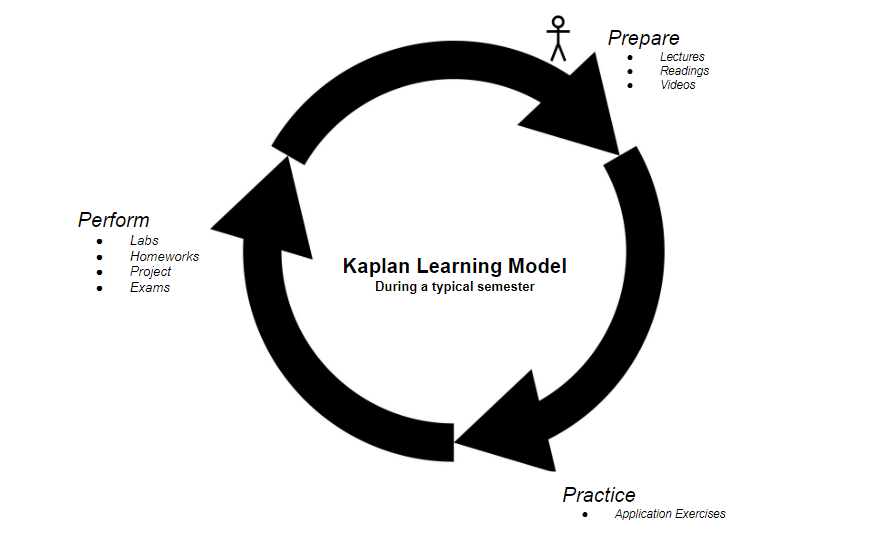
\includegraphics{images/Kaplan.png}

}

\end{figure}

This model is composed of three phases: prepare, practice, and perform.
All three phases are designed to guide the instructor in facilitating an
overall quality learning experience for the student. Each of these
phases are performed during a typical week within a semester, including
through preparation material, lectures, in-class application exercises,
labs, and assessments such as homework.

During the prepare phases, students are completing readings, watching
videos, and listening to lecture that ultimately builds upon a new
foundation of data science concepts being learned. The goal of preparing
students is to put them in a position where they can build upon what
they are learning, and create new knowledge through the practice phase.
The practice phase is designed to be an opportunity for students to
reinforce the new information gained, as well as uncover new concepts in
data science. This is achieved through the use of interactive
application exercises (AEs) in class where students work alone, in
groups, or with the instructor in live coding sessions. Finally,
students enter the perform phase to show their progress made in the
previous two phases. This is typically done through assessments such as
homework, exams, and projects. Additionally, students perform
individually, or with a group, during weekly labs that tend to focus
more on computation. This learning model is a continuous cycle
throughout the semester as new topics are introduced.

Topics taught in STA199 fall under two major units: Unit 1 - Exploring
data; Unit 2 - Making rigorous conclusions. In Unit 1, students become
first introduced to R, R-studio, and Github. During this unit, students
start to create data visualizations and learn how to both import and
manipulate data to be better suited for analysis. In unit 2, students
extend their investigations with data to include modeling. Specifically,
students fit a variety of models (simple linear regression, multiple
linear regression, logistic regression), and learn the fundamentals of
hypothesis testing. For a more complete description about the topics
taught and data sets used in creating these lessons, please see
\textbf{A fresh look at introductory data science (cite)}.

In this paper, we describe the preparation and implementation process of
STA199 in its entirety. This includes details of the teaching team used
to instruct STA199, technology chosen to use when creating and
facilitating our introductory data science course, and the pedagogical
choices that go into a typical week of teaching. This includes a
comprehensive description of a flexible framework on how to create, set
up, and implement an introduction to data science course similar to
STA199. When describing this framework, we articulate first hand
experiences and suggestions surrounding some of the choices made to
create and instruct STA199.

\hypertarget{teaching-team}{%
\section{Teaching Team}\label{teaching-team}}

We define a teaching team as a group consisting of one instructor and
multiple teaching assistants (TAs). The assignment of any teaching
assistant is to both support the instructor in charge of the class, and
support the students in the classroom. These TAs range from
undergraduate to PH.D. level students, and vary in teaching experience.
(Writing on TA selection process). Once selected\ldots{} (writing on TA
training).

Once training is complete, students are assigned roles that indicate
their responsibilities during the semester. These roles include
\emph{course organizer}, \emph{head TA}, \emph{lab leader}, and
\emph{lab helper}. Often, these roles are given based on the level of
student, with more academically experienced TAs taking on the roles of
course organizer, head TA, and lab leader, where as students with less
experience (i.e.~undergraduate students) take on the role of lab helper.

Lab sections are held once a week, and are facilitated in person by both
a lab leader and lab helper. The responsibilities of a lab helper are
supporting both the students and lab leader as they see fit. Examples of
this may include setting up the classroom before class, or conducting
small group conversations when students have questions about the
material. The lab leader is responsible for facilitating the lab. This
involves working through a pre-made lab to ensure they can help students
apply concepts discussed in lecture to what's being assigned. In
addition, both must hold two hours of office hours each week and have
grading responsibilities assigned throughout the semester.

Head TA responsibilities can generally be categorized as one of the
following: Administrative or Pedagogical. Administrative
responsibilities include the organization and distribution of TA
responsibilities throughout the semester. It is imperative that the head
TA and instructor clearly communicate expectations with each other to
establish exactly how rules and responsibilities that are given to the
TAs are assigned. Administrative duties include reminding other TAs
about bi-weekly payroll deadlines and ensure TAs are working their
alloted hours per week (and not more). Within these alloted hours, a
head TA distributes grading assignments and deadlines to both lab
helpers and leaders per week. They make sure all TAs complete grading
within a week and spot check the grading accuracy and quality of all
written feedback given. (insert 1-2 sentences about experience).
Pedagogically, head TAs are responsible for creating or reviewing answer
keys and grading rubrics for homework and lab assessments as the
instructor sees fit. Each head TA is also assigned to instruct one lab
section during the semester. Before becoming a Head TA, there are
additional

The course organizer is expected to work across each section of STA199,
instead of working with a single instructor. Their responsibilities
include creating rubrics for and working through homework and lab
assignments. Additionally the course organizer, along with the
instructor, answers real time questions virtually during labs from lab
leaders. Questions often range from content related to technical
questions about GitHub and R. Finally, the course organizer is
responsible for handling all requested assignment extension requests
from students. This includes filing away student exemptions, providing
extensions for extreme circumstances, and enforcing the late work policy
outlined in the syllabus when necessary.

(Paragraph on flexiability in team structure)

Through my experience as an instructor working with this designed team,
it is imperative that everyone is communicating with each other. A team
with many different roles poses risk for the instructor to be unaware of
how or what decisions are being enacted at the grading and lab levels of
the course. Thus, it is recommended that the instructor trains everyone
on the teaching team to use a communication system that allows every
member to communicate any questions they may have, or decisions they
make to the entire team. In the past, we have used the software
\emph{Slack}, with appropriately named channels such as
\emph{grading-questions} where TAs can post examples and questions about
grading and the instructor can clearly state their expectations.
Further, it should be noted that the head TA should not be treated as a
``bridge of communication'' for the instructor to the rest of the
teaching team. It is critical that that the instructor is in consistent
contact with all members of the teaching team in making sure all lab
leaders and helpers understand the course content, upcoming assignments,
and know what's expected of them in their assigned role. We recommend
holding a weekly meeting with all members of the teaching team to ensure
this. When members are unable to come, it is an expectation that they
watch a recorded video of the meeting and reach out if they have any
questions about what was discussed.

\hypertarget{sec-tech}{%
\section{Technology}\label{sec-tech}}

In this section we will detail the computing infrastructure used in
STA199 used to create and a course such as STA199. This includes details
on how to use R, R-studio, and GitHub's from the instructor's
perspective to set up lectures, AEs, labs and homework. First, we start
with the student information necessary to collect and steps that must be
taken before creation can take place.

\hypertarget{setting-up-a-github-account}{%
\subsection{Setting up a GitHub
account}\label{setting-up-a-github-account}}

We can use R, R-studio, and GitHub to create interactive lessons, and
assign pre-created assessments to individual or groups of students. To
do so, we must instruct students to create a GitHub account. This is
done of the first day of class, and often, students are given time
during class to sign up. Following tips from ``Happy Git with R''
(cite), we suggest students do the following when creating their name:

-- Incorporate your actual name -- Reuse your username from other
contexts if you can -- Pick a username you will be comfortable revealing
to your future boss -- Be as unique as possible in as few characters as
possible. Shorter is better than longer -- Avoid words with special
meaning in programming (i.e., NA)

Once students create their account, we suggest getting this information
from them in a survey. This normally can be done through your learning
management system. It is critical to reiterate to students that spelling
and capitalization matter when answer this question. We suggest asking
the question as follows: (insert question here).

If you, as the instructor, do not have a GitHub account, you will need
to create one as well. This student information will be needed to create
your GitHub organization for your course.

\hypertarget{github-organization}{%
\subsection{GitHub organization}\label{github-organization}}

GitHub organizations are shared accounts where instructors and students
can collaborate across many projects at once. Using your account, you
can create a new GitHub organization by clicking on your profile icon in
the upper right hand corner, go to \emph{Settings}, \emph{Access},
\emph{New Organization}. It's suggested to name this organization the
name of your class and the current semester you teaching in (i.e.,
sta199-s23). One of the many benefits of teaching through GitHub is the
ability to re-use what you currently create as a template for subsequent
semesters. Once your organization is created we can use packages within
R and R-studio to efficiently invite students and create assessments for
them.

\hypertarget{setting-up-r-r-studio}{%
\subsection{Setting Up R \& R-Studio}\label{setting-up-r-r-studio}}

R is a statistical programming language for computing, modeling, and
data visualization, while R-studio is an integrated development
environment for R (cite). Both are freely available to download and use.
In an introductory course, it is recommended to minimize student
frustration and distraction through the use of pre-packaged
computational infrastructure (Çetinkaya-Rundel and Rundel, 2018). Per
this recommendation, STA199 has students use R and R-studio through a
\emph{Duke Container}. Duke containers provides instructors at Duke
university the opportunity to facilitate the use of different software,
such as R and R-studio, through an online container instead of needing
students to locally download both programs. Additionally, instructors
have the ability to manage and install packages students will need for
the semester, helping provide a neat and well organized starting
experience with a new statistical language. (insert discussion on how
this is done).

(Thoughts: Transition to R-studio cloud discussion? What alternatives
can instructors use to imitate Duke containers if this is something they
do not have access to at their university.)

\hypertarget{using-r-r-studio-to-manage-organization}{%
\subsection{Using R \& R-Studio to manage
organization}\label{using-r-r-studio-to-manage-organization}}

(insert discussion / how-to on ghclass): includes invitations.

(set the stage for writing on how to create repos for students is
subsequent sections \emph{which will be a good segway})

R, R-studio, and GitHub aids in the creation and implementation our data
science pedagogy. This includes the creation and distribution of
in-class AEs, lectures, labs, and assessments. In the following sections
we describe in detail both how to create, structure, and distribute
materials used in STA199.

\begin{figure}

{\centering 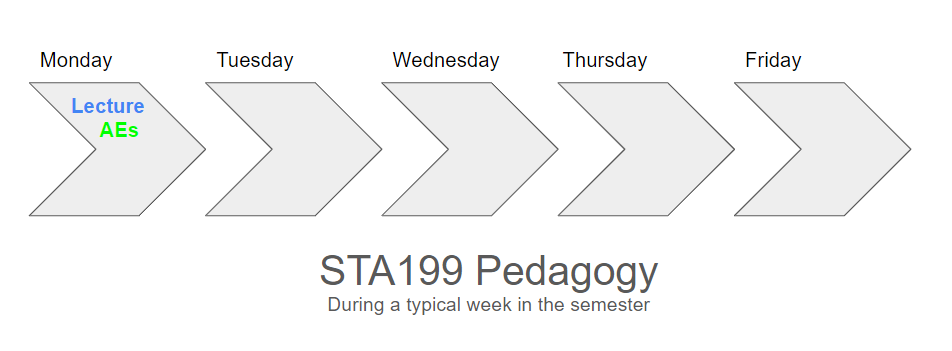
\includegraphics{images/pedagogy.png}

}

\end{figure}

Unpack the image below

\hypertarget{sec-ped}{%
\section{Pedagogy}\label{sec-ped}}

-- Reader should want to continue reading by thinking ``so how do I
teach this''

In this course, we have chosen a combination of teaching methods,
interactive activities, and learning assessments to help best prepare
introductory data science students the tools they need to be successful
outside of university or in future coursework. Our pedagogy includes
facilitating in-class AEs, facilitating lectures, running a lab, and
assigning assessments to provide students an opportunity to show what
they've learned.

\hypertarget{application-exercies-aes}{%
\subsection{Application Exercies (AEs)}\label{application-exercies-aes}}

A majority of the time in class will be dedicated to working on AEs.
These exercises are live-coding opportunities to practice applying data
science concepts and code introduced through preparation materials. AEs
are no-stakes assessments, often graded on completion, where students
have the ability to write and edit code while asking questions at the
student or class level and receive immediate feedback.

-- How GitHub and R are used to create AEs for students

It is up to the discretion of the instructor on the content that goes
into the AEs. This can include having students write code themselves,
fill in the blank coding exercises, commenting on complete code, or a
combination of such questions.

-- Kaplan Way (Practice) / Active learning implementation of AEs
(typical class day strategies / discussion)

\hypertarget{lecture}{%
\subsection{Lecture}\label{lecture}}

A typical week yields 75-minute lectures on Mondays and Wednesdays.
These lectures take up part of the class time, and are designed to
introduce new concepts or review topics from the preparation videos in a
more traditional format.

-- Creating slides using Quarto in R (?)

-- Kaplan Way (Prepare) / Active learning implementation during lecture
(typical class day strategies / discussion)

Lectures are recorded and made available to students with an excused
absence upon request.

\hypertarget{labs}{%
\subsection{Labs}\label{labs}}

-- apply the concepts discussed in lecture to various data analysis
scenarios, with a focus on the computation

-- Individual and team based

-- Repo creation

-- Kaplan Way (Perform) (typical class day strategies / discussion)

\hypertarget{assessments}{%
\subsection{Assessments}\label{assessments}}

-- Kaplan Way (Perform)

-- HW

\begin{itemize}
\tightlist
\item
  apply what you've learned during lecture and lab to complete data
  analysis tasks
\end{itemize}

-- Lab

\begin{itemize}
\item
  apply the concepts discussed in lecture to various data analysis
  scenarios, with a focus on the computation
\item
  Individual and team based
\item
  Repo creation
\end{itemize}

-- Exams

\begin{itemize}
\item
  opportunity to demonstrate what you've learned in the course thus far
\item
  take home exams
\end{itemize}

-- Project

\begin{itemize}
\item
  analyze an interesting data-driven research question
\item
  group project
\item
  describe the process / expectations of the project
\end{itemize}

\^{}\^{} The writing above should be in a form where there is practical
/ useful information for the reader. If they were designing the course,
do they better understand the assessment structure of an Intro to Data
Science course?

\hypertarget{discussion}{%
\section{Discussion}\label{discussion}}

It is imperative that universities create and implement modernized data
science curricula to both prepare and inspire students to continue their
data science education. This starts with the design and development of
an introductory data science course. At Duke University, the
technological preparations students receive in STA199 have pushed higher
level courses, such as courses in regression, to incorporate Quarto for
reproducibility and GitHub for collaboration and version control.

However, there is little consensus on the technological and
implementation procedures necessary to create and conduct a modernized
introductory data science course. We believe that the \emph{Introductory
to Data Science and Statistical Reasoning} helps establish a start to a
consensus while providing a flexible framework for other instructors to
create and facilitate their own introductory data science course.

It is highly advised that live coding sessions be the main staple of
your classroom when teaching students. Live coding sessions continue to
be accepted as one of the best pedagogical practices for teaching coding
(https://dl.acm.org/doi/abs/10.1145/3430665.3456382), and have been met
in our classrooms with overwhelming positivity from students: ``insert
more quotes.''

For this to successful, we suggest spending the first couple classes
establishing a routine with your students. This routine ensures that
students clone the live coding exercise (application exercise) prior to
the start of class, and understand that the expectation is to ``learn
through doing'' in live coding sessions.

Despite this suggestion, there are always situations where students can
fall behind in class, limiting the amount of value they may receive from
the day's lesson. Thus, we have come up with strategies to try and
mitigate the situation. First, the majority of student coding at the
beginning of the semester is done through fill in the blank templates
created by the instructor. This tends to ease tension for those first
learning code, and help instill confidence when the code runs. Secondly,
it is suggested to design questions in such a way where there is little
dependency across questions. This means that, if a student falls behind
and is unable to answer one question, this will not deter them from
being involved in upcoming questions. If you do have questions dependent
on each other, we advise providing the answers to the beginning
questions in the same or different document for students to reference
and run so they can continue following along.

With the time investment needed to create enticing and interactive AEs,
it is critical that these resources are easily transferable across
semesters. The design and facilitation of this course is through GitHub.
This ensures that the course content is feasible to adapt to teach for
multiple semesters as classes change and data science continues to
evolve. In short, there is value in the investment to quality resources
early in the classes development, saving time for future renditions.

Additional benefits in deciding to run the course through GitHub help
alleviate the burdens of large class sizes. Using the \texttt{ghclass}
package in R, an instructor can seamlessly distribute homework, labs,
and live coding exercises to as many students as necessary in little
time.

\hypertarget{supplementary-materials}{%
\section{Supplementary materials}\label{supplementary-materials}}

-- Pros (What works well)

Ex. Live coding good

-- Cons (What could be improved)

Ex. Students can fall behind during live coding sessions

-- Experiences

Examples include

-- Feasible to adopt to teach for multiple semesters as data science
continues to evolve. There is value in the investment.

-- Computational Resources

-- Human Resources

\newpage

the \emph{Kaplan Way}. The Kaplan Way is a learning model ``that
combines a scientific, evidence-based design philosophy with a
straightforward educational approach to learning''
\citep{schweser_2023}. This learning model posits a three-phase learning
strategy: Prepare, Practice, and Perform \textbf{TO DO: Check in with
Maria about provenance of PPP}. During each of these phases, students
are equipped with the appropriate tools to acquire knowledge, be given
an opportunity to apply what they know, and to demonstrate mastery of
the tasks at hand.


  \bibliography{bibliography.bib}


\end{document}
